\documentclass[a4paper,12pt]{extarticle}
\usepackage[utf8x]{inputenc}
\usepackage[T1,T2A]{fontenc}
\usepackage[russian]{babel}
\usepackage{hyperref}
\usepackage{indentfirst}
\usepackage{listings}
\usepackage{color}
\usepackage{here}
\usepackage{array}
\usepackage{multirow}
\usepackage{graphicx}
\usepackage{amsmath}
\usepackage{amssymb}

\usepackage{caption}
\renewcommand{\lstlistingname}{Программа} % заголовок листингов кода

\bibliographystyle{ugost2008ls}

\usepackage{listings}
\lstset{ %
extendedchars=\true,
keepspaces=true,
language=C,						% choose the language of the code
basicstyle=\footnotesize,		% the size of the fonts that are used for the code
numbers=left,					% where to put the line-numbers
numberstyle=\footnotesize,		% the size of the fonts that are used for the line-numbers
stepnumber=1,					% the step between two line-numbers. If it is 1 each line will be numbered
numbersep=5pt,					% how far the line-numbers are from the code
backgroundcolor=\color{white},	% choose the background color. You must add \usepackage{color}
showspaces=false				% show spaces adding particular underscores
showstringspaces=false,			% underline spaces within strings
showtabs=false,					% show tabs within strings adding particular underscores
frame=single,           		% adds a frame around the code
tabsize=2,						% sets default tabsize to 2 spaces
captionpos=t,					% sets the caption-position to top
breaklines=true,				% sets automatic line breaking
breakatwhitespace=false,		% sets if automatic breaks should only happen at whitespace
escapeinside={\%*}{*)},			% if you want to add a comment within your code
postbreak=\raisebox{0ex}[0ex][0ex]{\ensuremath{\color{red}\hookrightarrow\space}},
texcl=true,
inputpath=listings,                     % директория с листингами
}

\usepackage[left=2cm,right=2cm,
top=2cm,bottom=2cm,bindingoffset=0cm]{geometry}

%% Нумерация картинок по секциям
\usepackage{chngcntr}
\counterwithin{figure}{subsection}
\counterwithin{table}{section}

%%Точки нумерации заголовков
\usepackage{titlesec}
\titlelabel{\thetitle.\quad}
\usepackage[dotinlabels]{titletoc}

%% Оформления подписи рисунка
\addto\captionsrussian{\renewcommand{\figurename}{Рис.}}
\captionsetup[figure]{labelsep = period}

%% Подпись таблицы
\DeclareCaptionFormat{hfillstart}{\hfill#1#2#3\par}
\captionsetup[table]{format=hfillstart,labelsep=newline,justification=centering,skip=-10pt,textfont=bf}

%% Путь к каталогу с рисунками
\graphicspath{{fig/}}

\begin{document}	% начало документа
\setcounter{tocdepth}{3}

% Титульная страница
\begin{titlepage}	% начало титульной страницы

	\begin{center}		% выравнивание по центру

		\large Санкт-Петербургский Политехнический Университет Петра Великого\\
		\large Институт компьютерных наук и технологий \\
		\large Кафедра компьютерных систем и программных технологий\\[6cm]
		% название института, затем отступ 6см
		
		\huge Телекоммуникационные технологии\\[0.5cm] % название работы, затем отступ 0,5см
		\large Отчет по лабораторной работе №7\\[0.1cm]
		\large Помехоустойчивое кодирование\\[5cm]

	\end{center}


	\begin{flushright} % выравнивание по правому краю
		\begin{minipage}{0.25\textwidth} % врезка в половину ширины текста
			\begin{flushleft} % выровнять её содержимое по левому краю

				\large\textbf{Работу выполнил:}\\
				\large Болдырев А.В.\\
				\large {Группа:} 33501/3\\
				
				\large \textbf{Преподаватель:}\\
				\large Богач Н.В.

			\end{flushleft}
		\end{minipage}
	\end{flushright}
	
	\vfill % заполнить всё доступное ниже пространство

	\begin{center}
	\large Санкт-Петербург\\
	\large \the\year % вывести дату
	\end{center} % закончить выравнивание по центру

\thispagestyle{empty} % не нумеровать страницу
\end{titlepage} % конец титульной страницы

\vfill % заполнить всё доступное ниже пространство

% Содержание
% Содержание
\renewcommand\contentsname{\centerline{Содержание}}
\tableofcontents
\newpage


\section{Цель и задачи}

\subsection{Цель работы}
Изучение методов помехоустойчивого кодирования и сравнения их свойств.
 
\subsection{Постановка задачи}
Провести кодирование/декодирование сигнала, полученного с помощью функции randerr кодом Хэмминга 2-мя способами: с помощью встроенных функций encode/decode, а также через создание проверочной и генераторной матриц и вычисление синдрома. Оценить корректирующую способность кода.

Выполнить кодирование/декодирование циклическим кодом, кодом БЧХ, кодом Рида-Соломона. Оценить корректирующую способность кода.

 
\section{Теоретическая информация}

\subsection{Кодирование}
Физическое кодирование — линейное преобразование двоичных данных, осуществляемое для их передачи по физическому каналу (такому как оптическое волокно или витая пара). Физическое кодирование может менять форму, ширину полосы частот и гармонический состав сигнала в целях осуществления синхронизации приёмника и передатчика, устранения постоянной составляющей или уменьшения аппаратных затрат.

Обнаружение ошибок в технике связи — действие, направленное на контроль целостности данных при записи/воспроизведении информации или при её передаче по линиям связи. Исправление ошибок (коррекция ошибок) — процедура восстановления информации после чтения её из устройства хранения или канала связи.

Для обнаружения ошибок используют коды обнаружения ошибок, для исправления — корректирующие коды (коды, исправляющие ошибки, коды с коррекцией ошибок, помехоустойчивые коды).

\subsection{Типы помехоустойчивого кодирования}
\subsubsection{Кодирование Хэмминга}
Коды Хемминга — простейшие линейные коды с минимальным расстоянием 3, то есть способные исправить одну ошибку. Код Хемминга может быть представлен в таком виде, что синдром

\begin{equation}
\vec{s} = \vec{r} H^T
\end{equation}

Это принятый вектор, будет равен номеру позиции, в которой произошла ошибка. Это свойство позволяет сделать декодирование очень простым.

Коды Хэмминга являются самоконтролирующимися кодами, то есть кодами, позволяющими автоматически обнаруживать ошибки при передаче данных. Для их построения достаточно приписать к каждому слову один добавочный (контрольный) двоичный разряд и выбрать цифру этого разряда так, чтобы общее количество единиц в изображении любого числа было, например, нечетным. Одиночная ошибка в каком-либо разряде передаваемого слова (в том числе, может быть, и в контрольном разряде) изменит четность общего количества единиц. Счетчики по модулю 2, подсчитывающие количество единиц, которые содержатся среди двоичных цифр числа, могут давать сигнал о наличии ошибок.

При этом невозможно узнать, в каком именно разряде произошла ошибка, и, следовательно, нет возможности исправить её. Остаются незамеченными также ошибки, возникающие одновременно в двух, четырёх, и т. д. — в четном количестве разрядов. Впрочем, двойные, а тем более четырёхкратные ошибки полагаются маловероятными.

Коды, в которых возможно автоматическое исправление ошибок, называются самокорректирующимися. Для построения самокорректирующегося кода, рассчитанного на исправление одиночных ошибок, одного контрольного разряда недостаточно. Как видно из дальнейшего, количество контрольных разрядов k должно быть выбрано так, чтобы удовлетворялось неравенство 
\begin{equation}
2^{k}\geq k+m+1
\end{equation}
или  
\begin{equation}
k \geq \log _{2}(k+m+1) 
\end{equation}

где m — количество основных двоичных разрядов кодового слова.

Минимальные значения k при заданных значениях m, найденные в соответствии с этим неравенством, приведены в таблице.
\begin{figure}[H]
	\begin{center}
		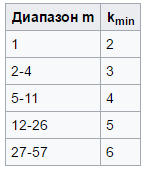
\includegraphics[width=0.2\linewidth]{Table_kmin.png}
		\caption{Значения $K_{min}$ в зависимости от $m$.} %% подпись к рисунку
		\label{Table_kmin} %% метка рисунка для ссылки на него
	\end{center}
\end{figure}

В настоящее время наибольший интерес представляют двоичные блочные корректирующие коды. При использовании таких кодов информация передаётся в виде блоков одинаковой длины и каждый блок кодируется и декодируется независимо друг от друга. Почти во всех блочных кодах символы можно разделить на информационные и проверочные. Таким образом, все комбинации кодов разделяются на разрешенные (для которых соотношение информационных и проверочных символов возможно) и запрещенные.

Построение кодов Хэмминга основано на принципе проверки на четность числа единичных символов: к последовательности добавляется такой элемент, чтобы число единичных символов в получившейся последовательности было четным.

\begin{equation}
	r_1 = i_1 \oplus i_2 \oplus ... \oplus i_k
\end{equation}
где $\oplus$ - операция XOR.

\begin{equation}
	S = i_1 \oplus i_2 \oplus ... \oplus i_n \oplus r_1
\end{equation}
Тогда если $S = 0$ - ошибки нет, иначе есть однократная ошибка.

Такой код называется $(k+1,k)$ или $(n,n-1)$ . Первое число — количество элементов последовательности, второе — количество информационных символов.

Для каждого числа проверочных символов $ r=3,4,5..$ существует классический код Хэмминга с маркировкой $(n,k)=(2^{r}-1,2^{r}-1-r)$, то есть — $(7,4),(15,11),(31,26)$ . При иных значениях k получается так называемый усеченный код, например международный телеграфный код МТК-2, у которого $k=5$. Для него необходим код Хэмминга $(9,5)$, который является усеченным от классического $(15,11)$.

Для примера рассмотрим классический код Хемминга $(7,4)$. Сгруппируем проверочные символы следующим образом:

\begin{equation}
r_1 = i_1 \oplus i_2 \oplus i_3
r_2 = i_2 \oplus i_3 \oplus i_4
r_3 = i_1 \oplus i_2 \oplus i_4
\end{equation}

Получение кодового слова выглядит следующим образом:

\begin{equation}
( i_1 \> i_2 \> i_3 \> i_4 )  \begin{pmatrix}
1 & 0 & 0 & 0 & 1 & 0 & 1 \\
0 & 1 & 0 & 0 & 1 & 1 & 1 \\         
0 & 0 & 1 & 0 & 1 & 1 & 0 \\
0 & 0 & 0 & 1 & 0 & 1 & 1
\end{pmatrix} = ( i_1 \> i_2 \> i_3 \> i_4  \> r_1  \> r_2  \> r_3)
\end{equation}

На вход декодера поступает кодовое слово $V = (i_{1}', i_{2}', i_{3}', i_{4}', r_{1}', r_{2}', r_{3}')$  где штрихом помечены символы, которые могут исказиться в результате помехи. В декодере в режиме исправления ошибок строится последовательность синдромов:

$S_{1}=r_{1}\oplus i_{1}\oplus i_{2}\oplus i_{3}$

$S_{2}=r_{2}\oplus i_{2}\oplus i_{3}\oplus i_{4}$

$S_{3}=r_{3}\oplus i_{1}\oplus i_{2}\oplus i_{4}$

$S=(S_{1},S_{2},S_{3})$ называется синдромом последовательности.

Получение синдрома выглядит следующим образом:

\begin{equation}
(i_{1} \> i_{2} \> i_{3} \> i_{4} \> r_{1} \> r_{2} \> r_{3} )  \begin{pmatrix}
1 & 0 & 1 \\
1 & 1 & 1 \\
1 & 1 & 0 \\
0 & 1 & 1 \\
1 & 0 & 0 \\
0 & 1 & 0 \\
0 & 0 & 1 \\ 
\end{pmatrix} = \begin{pmatrix}S_{1}&S_{2}&S_{3}\\\end{pmatrix}
\end{equation}

Кодовые слова $(7,4)$ кода Хэмминга:

\begin{figure}[H]
	\begin{center}
		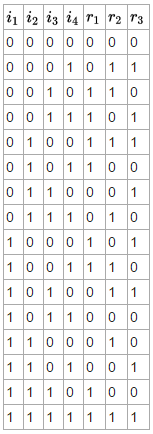
\includegraphics[width=0.2\linewidth]{Table_i_r.png}
		\caption{Кодовые слова $(7,4)$ кода Хэмминга.} %% подпись к рисунку
		\label{Table_i_r} %% метка рисунка для ссылки на него
	\end{center}
\end{figure}

Синдром $(0,0,0)$ указывает на то, что в последовательности нет искажений. Каждому ненулевому синдрому соответствует определенная конфигурация ошибок, которая исправляется на этапе декодирования.

Для кода $(7,4)$ в таблице указаны ненулевые синдромы и соответствующие им конфигурации ошибок (для вида: $i_1  i_2  i_3  i_4 r_1 r_2 r_3$).

\begin{figure}[H]
	\begin{center}
		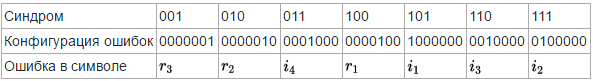
\includegraphics[width=0.8\linewidth]{Table_synd.png}
		\caption{Ненулевые синдромы для различных конфигураций ошибок в сообщении.} %% подпись к рисунку
		\label{Table_synd} %% метка рисунка для ссылки на него
	\end{center}
\end{figure}

\begin{figure}[H]
	\begin{center}
		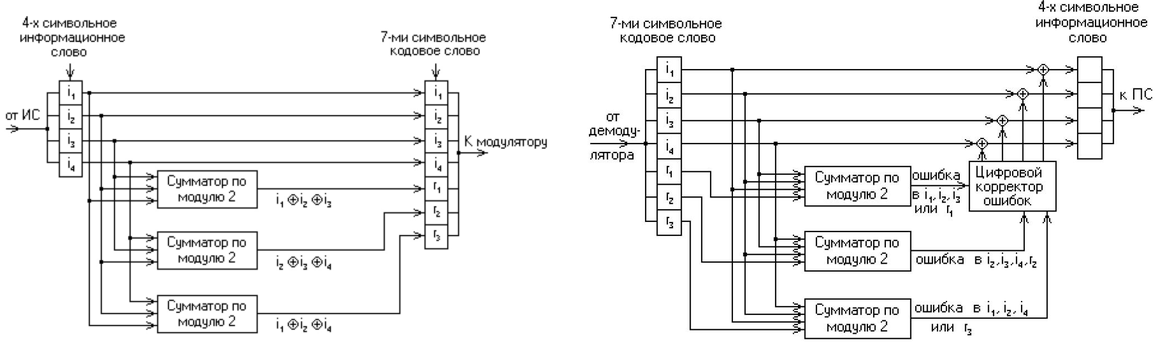
\includegraphics[width=1\linewidth]{Ham_De_Coder.png}
		\caption{Устройство кодера/декодера Хэмминга.} %% подпись к рисунку
		\label{Ham_De_Coder} %% метка рисунка для ссылки на него
	\end{center}
\end{figure}



\subsubsection{Циклические коды}
Циклический код — линейный код, обладающий свойством цикличности, то есть каждая циклическая перестановка кодового слова также является кодовым словом. Используется для преобразования информации для защиты её от ошибок.

\subsubsection{Коды Боуза-Чоудхури-Хоквингема (БЧХ)}
Коды Боуза — Чоудхури — Хоквингема (БЧХ-коды) — в теории кодирования это широкий класс циклических кодов, применяемых для защиты информации от ошибок. Отличается возможностью построения кода с заранее определёнными корректирующими свойствами, а именно, минимальным кодовым расстоянием. Частным случаем БЧХ-кодов является код Рида — Соломона.

\subsubsection{Коды Рида-Соломона}
Коды Рида — Соломона (англ. Reed–Solomon codes) — недвоичные циклические коды, позволяющие исправлять ошибки в блоках данных. Элементами кодового вектора являются не биты, а группы битов (блоки). Очень распространены коды Рида — Соломона, работающие с байтами (октетами).

Код Рида — Соломона является частным случаем БЧХ-кода.

В настоящее время широко используется в системах восстановления данных с компакт-дисков, при создании архивов с информацией для восстановления в случае повреждений, в помехоустойчивом кодировании.

\section{Ход работы}

Реализация различных типов кодирования с помощью MATLAB:
\lstinputlisting[
	label=code:code,
	caption={Код в МатЛаб},% для печати символ '_' требует выходной символ '\'
]{Code.m}

\subsection{Коды Хэмминга}

\subsection{Циклические коды}

\subsection{Коды Боуза-Чоудхури-Хоквингема (БЧХ)}

\subsection{Коды Рида-Соломона}


\section{Выводы}
Кодирование - важный процесс при передаче сигналов по каналам связи. Методы кодирования дополняют методы модуляции для обеспечения улучшения качества передачи, для предотвращения ошибок при передаче, а также защищенности данных от получения злоумышлинниками.
Рассмотрены различные методы кодирования - коды Хэмминга, циклические коды, коды Боуза-Чоудхури-Хоквингема, коды Рида-Соломона. 

\end{document}
